\chapter{Introduction}\label{chapter:intro}
FILL

\section{Problem Formulation}
The work presented in this thesis has in particular focused on the following research questions:
\begin{enumerate}
	\item[\textbf{Q1.}] Q1? Learn a scalable policy that is able to handle different scenarios 
	\item[\textbf{Q2.}] Q2? How can we combine MPC and RL? 
	\item[\textbf{Q3.}] Q3? estimate Uncertainty of the decisions and intentions.
\end{enumerate}



\begin{enumerate}
	\item We want to drive through intersections. 
	\item The intersection can be of different shapes. We assume we have a map of the intersection. 
	\item There will be other cars crossing the same intersection. 
	\item We have access to sensors on-board the ego vehicle. 
	\item We dont assume any knowlage of traffic signs or traffic lights. 
	\item We dont have v2v, or v2x communication. 
	
	To compensate for not having v2v or v2x communitaion, we have to predict what other driver will do. 
	
\end{enumerate}



\subsection{Scope / Limitations}
FILL

\subsection{System Architecture}
outline system architecture and limit this papre to comfortable decisions 

\begin{figure}[t]
	\centering
	\mbox{\parbox{\textwidth}{
			\centering
			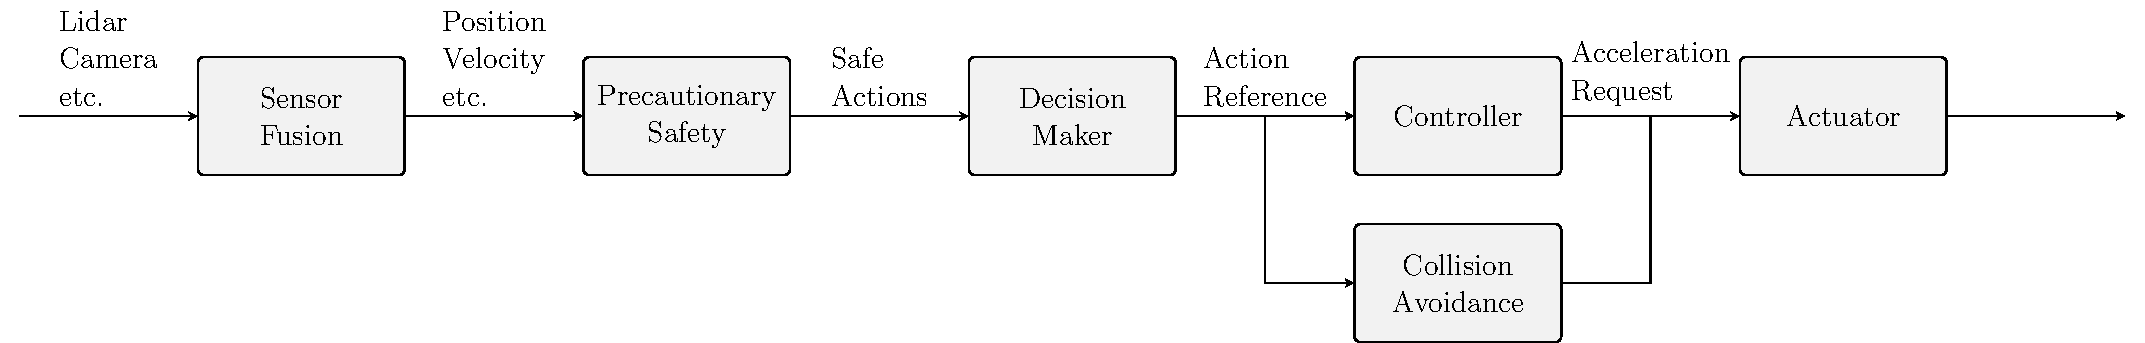
\includegraphics[width=\linewidth]{YourThesis/chapters/figures/pomdp/figures-system_architecture.pdf}%We suggest that you use a text box to insert a graphic (which is ideally a 300 dpi TIFF or EPS file, with all fonts embedded) because, in an document, this method is somewhat more stable than directly inserting a picture.   
	}}
	\caption{Representation of the system architecture.
	}
	\label{fig:systemArchitecture}
\end{figure}

\subsection{Contributions}

The main contributions of this thesis are:
\begin{enumerate}
	\item FILL

\end{enumerate}


\section{Thesis Outline}
FILL


